\chapter{Protótipo Interativo}

O protótipo interativo do \textit{GrabATable} foi desenvolvido no Figma~\cite{figma} e traduz o sistema visual definido na secção~\ref{sec:sistema-visual} (paleta, tipografia e componentes) em ecrãs navegáveis para os três perfis de utilizador. Para realizar os testes foi utilizado um iphone 13 pro.

\section{Acesso ao Protótipo}

O protótipo pode ser consultado e navegado através da seguinte ligação:

\begin{center}
  \href{https://www.figma.com/design/aaighKLXiie4lkBFsrhHsu/GrabATable?m=auto&t=5WWq2U1SLjYclMoF-1}{Abrir o protótipo no Figma}
\end{center}


\section{Fluxos de Interação}

Para cada perfil são apresentados dois fluxos: uma \textbf{tarefa principal},
correspondente à tarefa específica modelada na secção~\ref{sec:task-model} (\textit{Task Model}), e uma
\textbf{tarefa secundária}, que mostra uma funcionalidade complementar do mesmo perfil.
Cada figura mostra, ecrã a ecrã, a sequência de interações, com os toques assinalados a
dourado e uma legenda por passo.

\subsection{Administrador}

\subsubsection{Tarefa principal -- Adicionar um restaurante.}
Corresponde ao processo de adicionar um restaurante à plataforma que foi desenhado no \textit{Task Model} principal do administrador. O administrador inicia sessão, abre o separador Restaurantes, preenche os dados do restaurante e cria a conta do gestor em dois passos, e confirma a publicação no catálogo (RF13).

\begin{figure}[H]
  \centering
  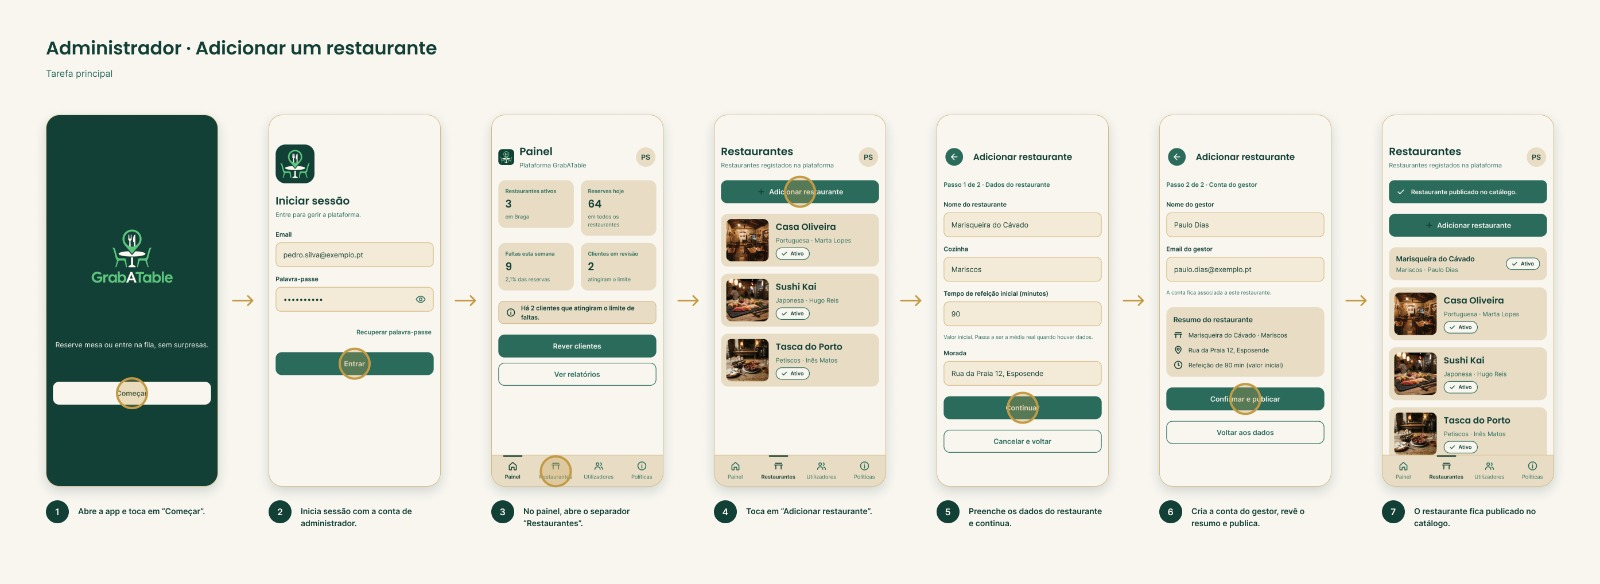
\includegraphics[width=\textwidth]{images/admin_principal.jpg}
  \caption{Administrador -- Adicionar um restaurante (tarefa principal)}
  \label{fig:proto-admin-principal}
\end{figure}

\subsubsection{Tarefa secundária -- Rever e bloquear um cliente.}
A partir do aviso no painel, o administrador abre a lista de clientes \textit{Em revisão},
consulta as faltas do cliente e confirma o bloqueio, sendo enviado um email ao cliente
(RF14). A ação é reversível através do botão \textit{Desbloquear cliente}.

\begin{figure}[H]
  \centering
  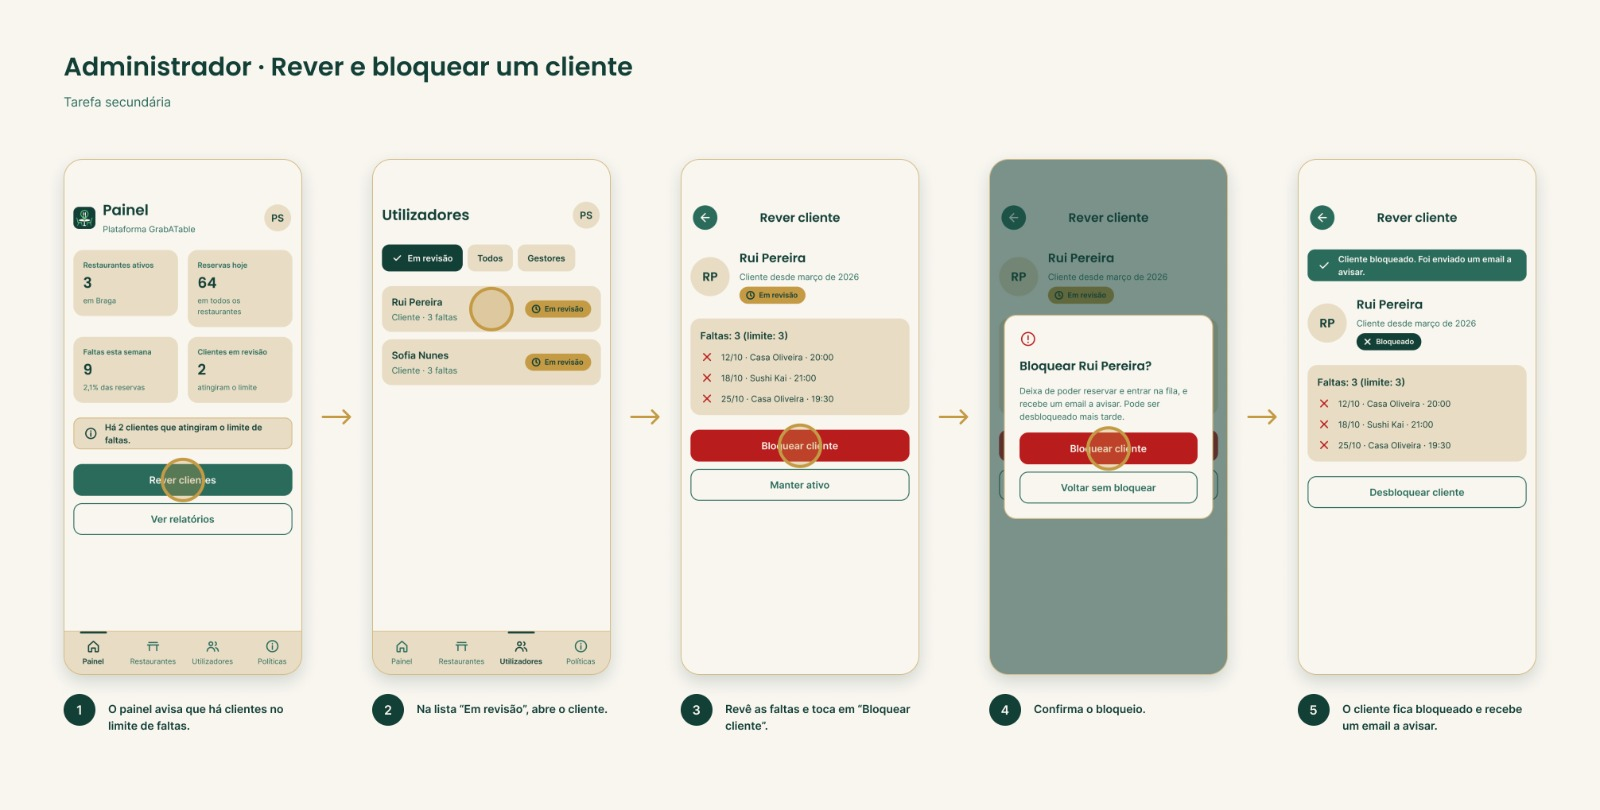
\includegraphics[width=\textwidth]{images/admin_secundario.jpg}
  \caption{Administrador -- Rever e bloquear um cliente (tarefa secundária)}
  \label{fig:proto-admin-secundario}
\end{figure}

\subsection{Gestor}

\subsubsection{Tarefa principal -- Atender um cliente com reserva.}
Corresponde ao processo de atender um cliente com reserva que foi desenhado no \textit{Task Model} principal do gestor. No painel de serviço, o gestor vê a próxima chegada, marca a chegada do cliente e confirma a mesa sugerida pelo sistema, que passa a ficar ocupada (RF09).

\begin{figure}[H]
  \centering
  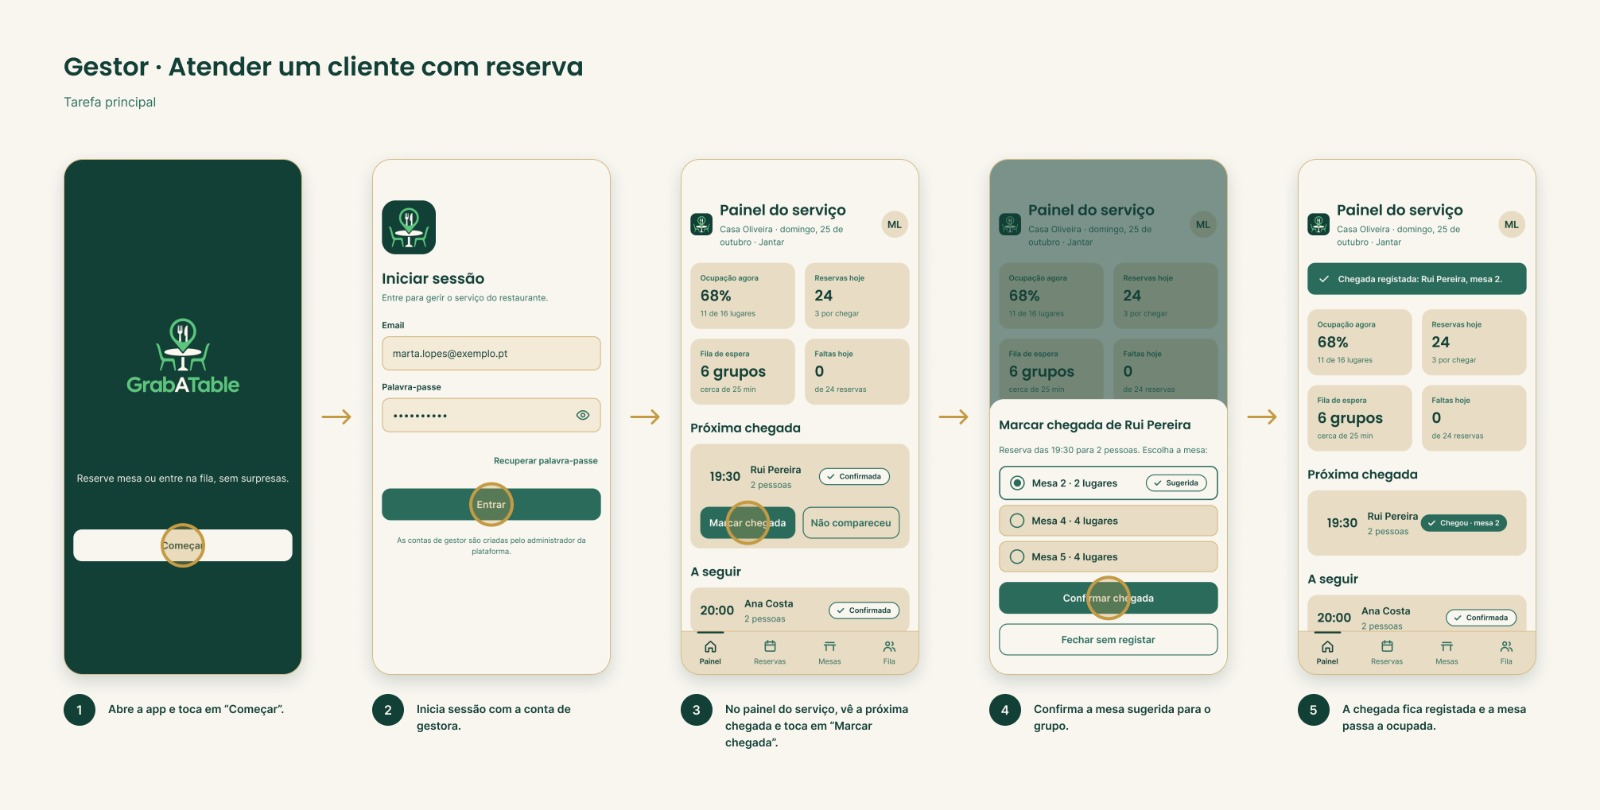
\includegraphics[width=\textwidth]{images/gestor_principal.jpg}
  \caption{Gestor -- Atender um cliente com reserva (tarefa principal)}
  \label{fig:proto-gestor-principal}
\end{figure}

\subsubsection{Tarefa secundária -- Libertar uma mesa.}
Quando o grupo sai, o gestor abre o separador \textit{Mesas} e liberta a mesa com dois
toques. O sistema avisa automaticamente o primeiro grupo da fila de espera que cabe nessa
mesa (RF10), o que mantém a estimativa de espera atualizada.

\begin{figure}[H]
  \centering
  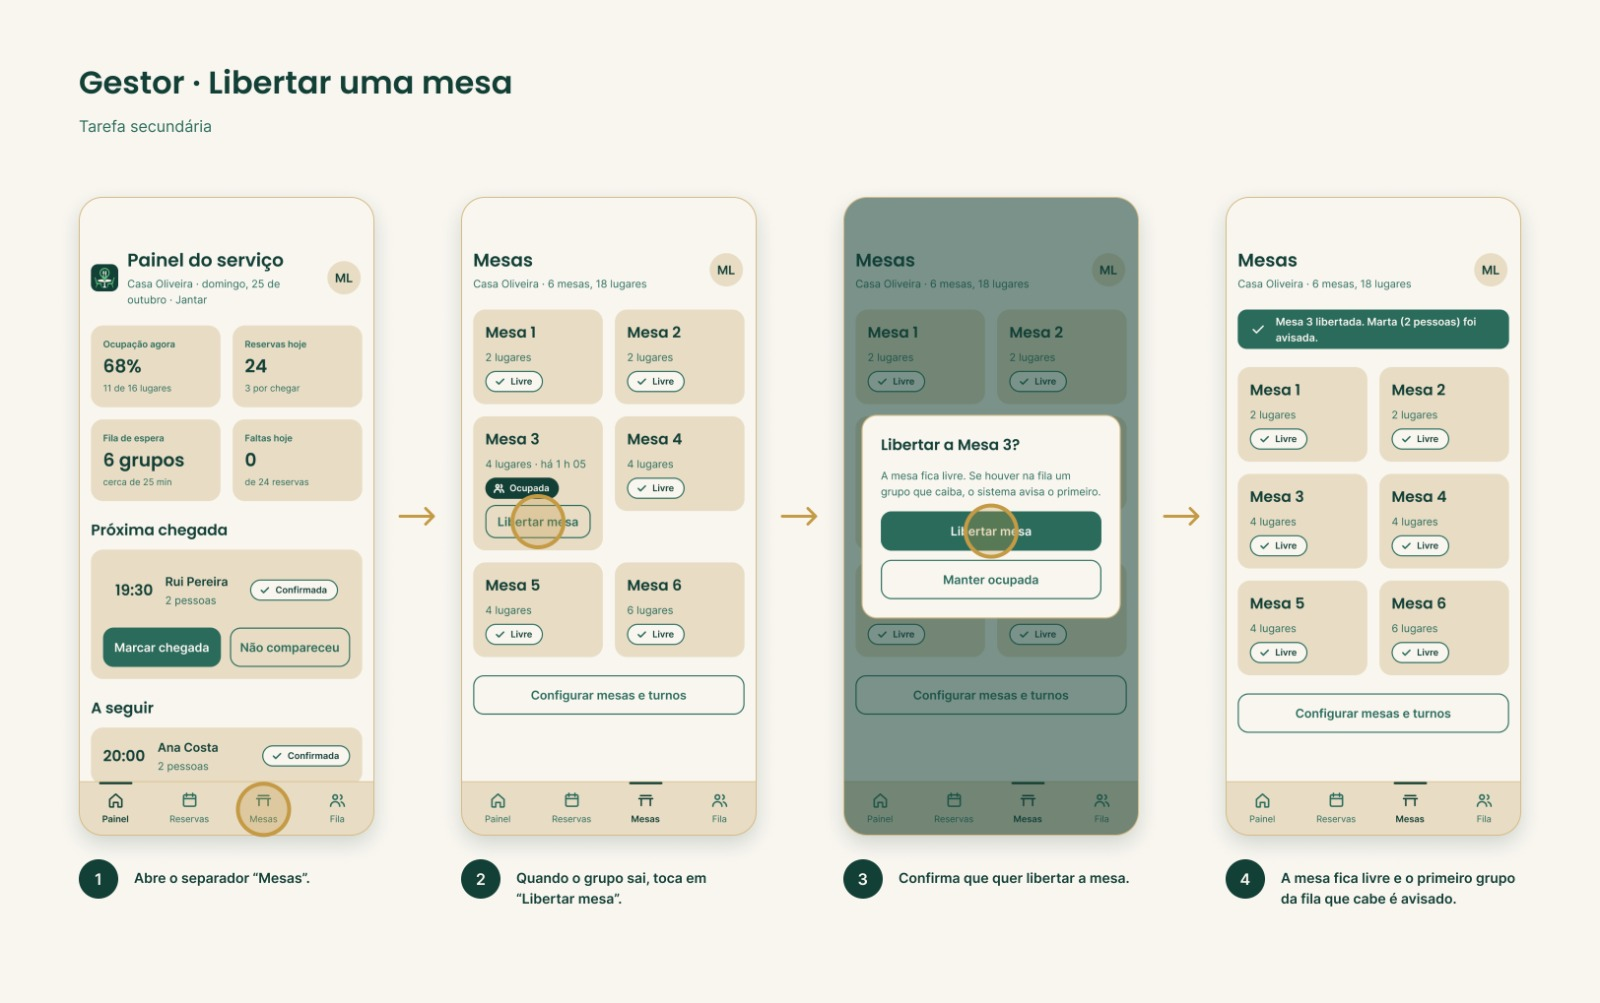
\includegraphics[width=\textwidth]{images/gestor_secundario.jpg}
  \caption{Gestor -- Libertar uma mesa (tarefa secundária)}
  \label{fig:proto-gestor-secundario}
\end{figure}

\subsection{Cliente}

\subsubsection{Tarefa principal -- Reservar mesa para refeição.}
Corresponde ao processo de reservar mesa para uma refeição que foi desenhado no \textit{Task Model} principal do cliente. O cliente inicia sessão, escolhe o restaurante, seleciona o dia, a hora e o número de pessoas e recebe a confirmação da reserva por email (RF03, RF04, RF05 e RF08).

\begin{figure}[H]
  \centering
  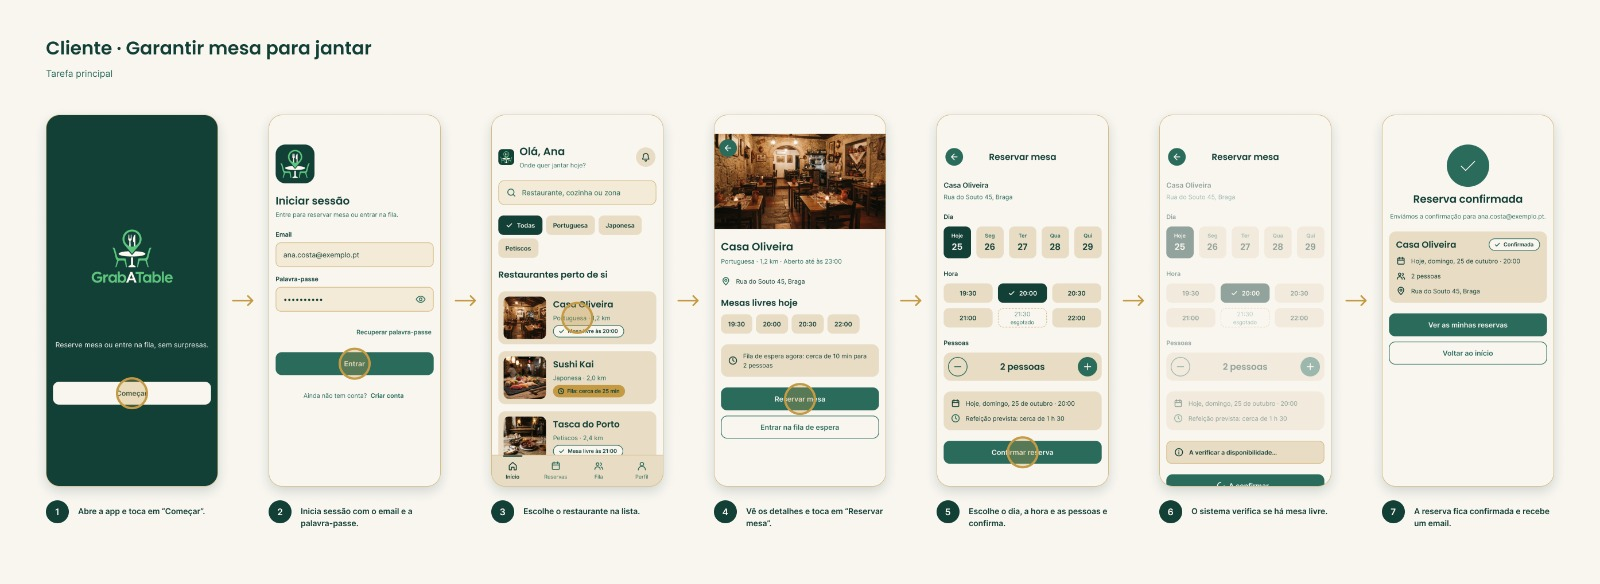
\includegraphics[width=\textwidth]{images/cliente_principal.jpg}
  \caption{Cliente -- Reservar mesa para refeição (tarefa principal)}
  \label{fig:proto-cliente-principal}
\end{figure}

\subsubsection{Tarefa secundária -- Entrar na fila de espera.}
Para o cliente sem reserva, o fluxo permite entrar na fila, ver o tempo estimado, acompanhar
a posição em tempo real e receber o aviso de que a mesa está quase pronta (RF07 e RF08).

\begin{figure}[H]
  \centering
  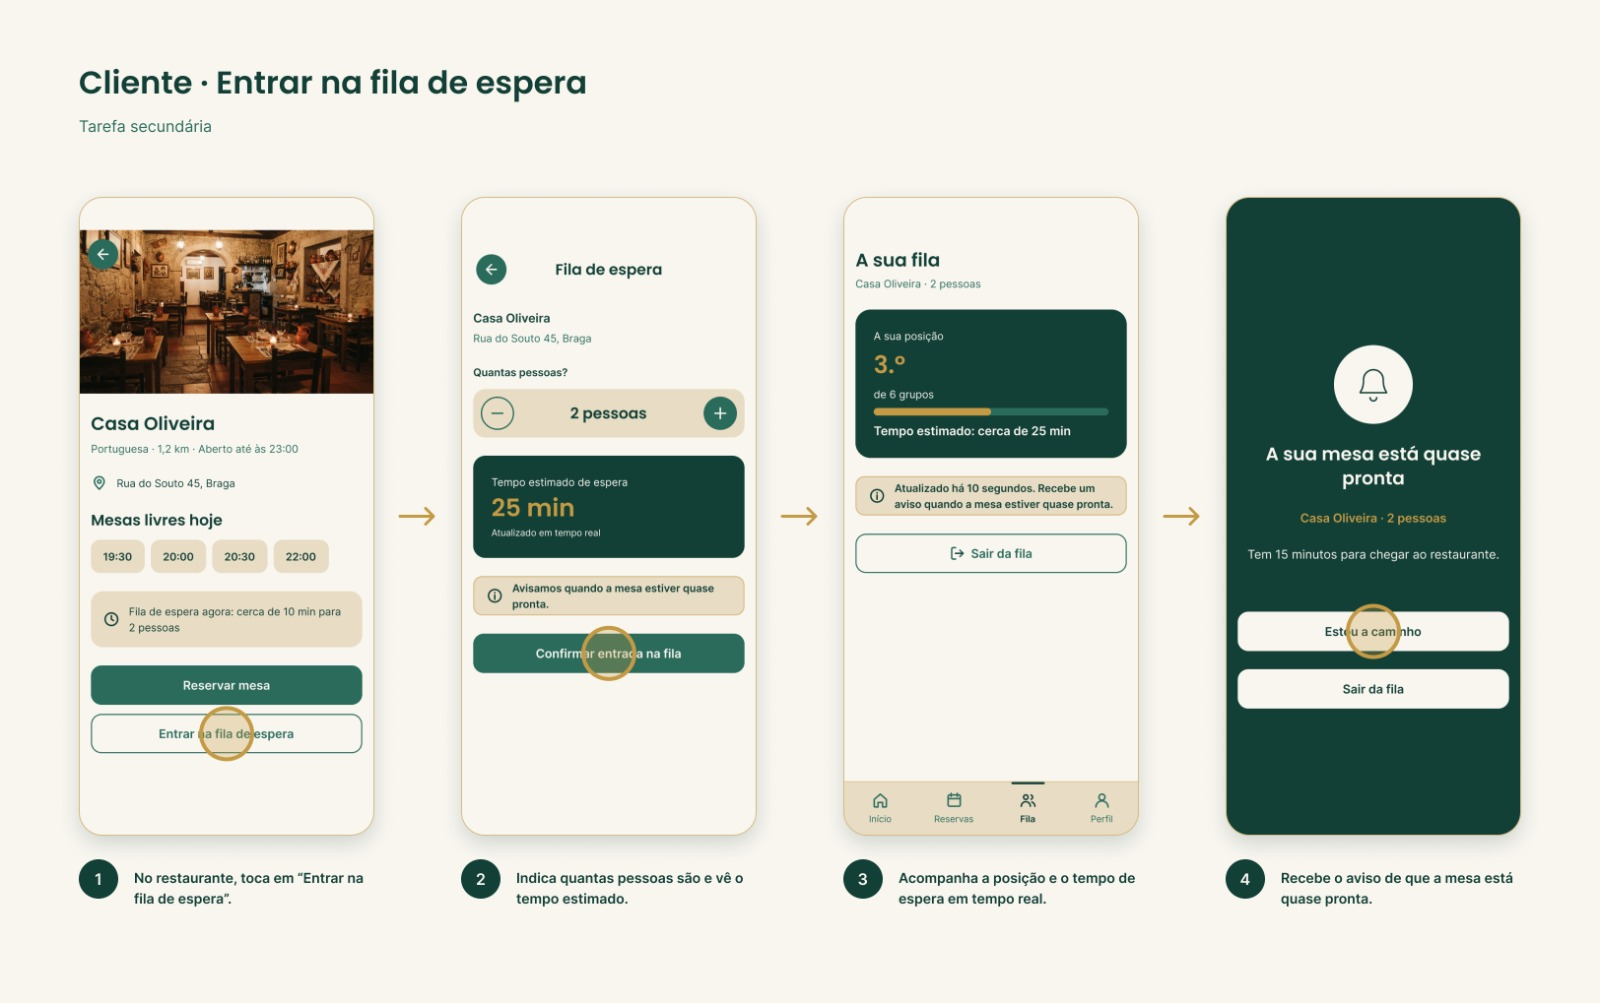
\includegraphics[width=\textwidth]{images/cliente_secundario.jpg}
  \caption{Cliente -- Entrar na fila de espera (tarefa secundária)}
  \label{fig:proto-cliente-secundario}
\end{figure}

\section{Vídeo de Demonstração}

Foi gravado um vídeo que demonstra a execução completa da tarefa principal definida para a aplicação. O vídeo está disponível em: \textit{(clicar na imagem em baixo)}

\href{https://youtube.com/shorts/b33i4PHJjyE?feature=share}{
    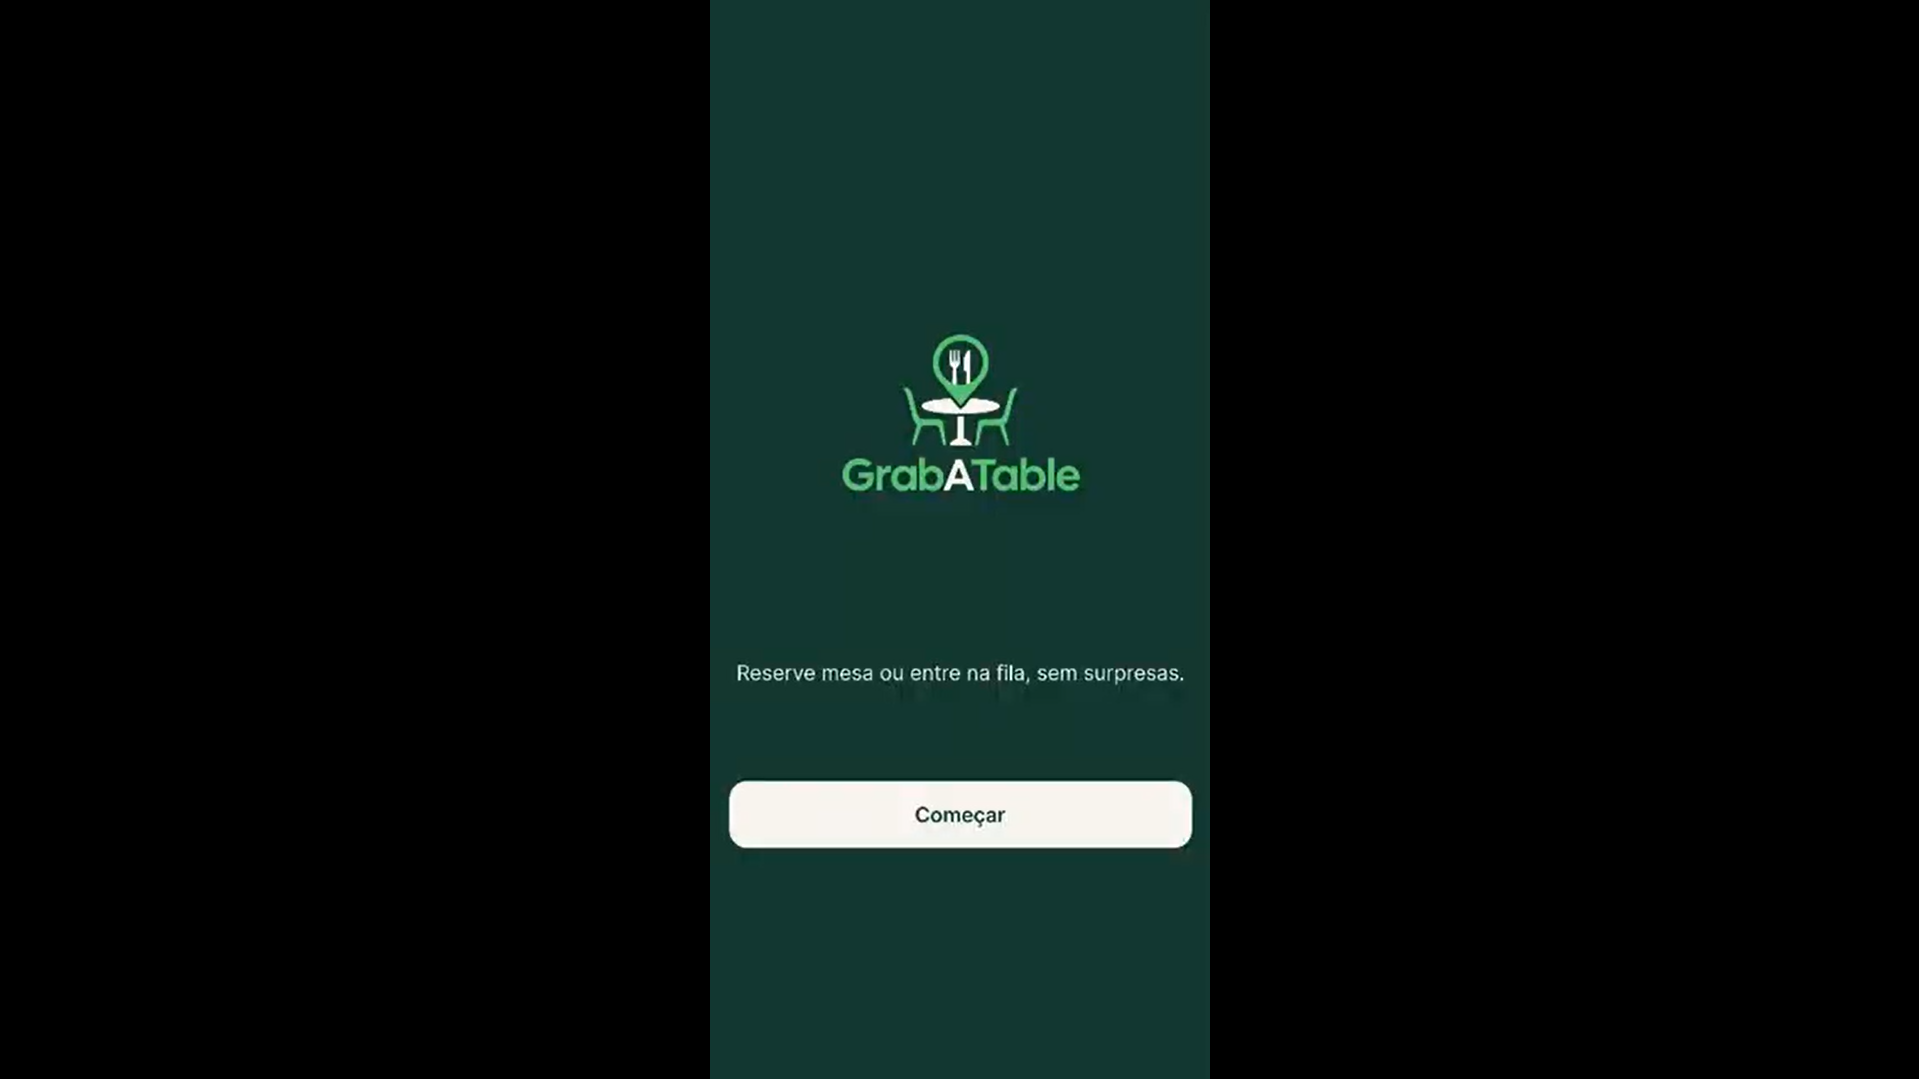
\includegraphics[width=0.9\textwidth]{images/video_foto.png}
}